\usetikzlibrary{shapes.geometric, arrows}

\tikzstyle{startstop} = [rectangle, rounded corners,
minimum width=3cm,
minimum height=1cm,
text centered,
draw=black,
fill=red!30]

\tikzstyle{io} = [trapezium,
trapezium stretches=true, % A later addition
trapezium left angle=70,
trapezium right angle=110,
minimum width=3cm,
minimum height=1cm, text centered,
draw=black, fill=blue!30]

\tikzstyle{process} = [rectangle,
minimum width=3cm,
minimum height=1cm,
text centered,
text width=3cm,
draw=black,
fill=orange!30]

\tikzstyle{decision} = [diamond,
minimum width=3cm,
minimum height=1cm,
text centered,
draw=black,
fill=green!30]
\tikzstyle{arrow} = [thick,->,>=stealth]

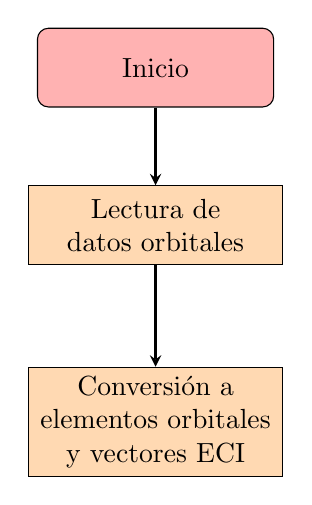
\begin{tikzpicture}[node distance=2cm]

    \node (start) [startstop] {Inicio};
    \node (pro1) [process, below of=start] {Lectura de datos orbitales};
    \node (pro2) [process, below of=pro1, yshift=-0.5cm] {Conversión a elementos orbitales y vectores ECI};

    \draw [arrow] (start) -- (pro1);
    \draw [arrow] (pro1) -- (pro2);

\end{tikzpicture}
